

\chapter{Quickstart}
\label{chap:Quickstart}
The aim of this chapter is to get a new TROVE user, especially PhD students and postdocs, up 
and running with the program to enable them to start carrying out calculations. 
It is assumed that for the molecule of interest, the molecular symmetry and geometric transforms have already been defined 
and that a PES and DMS has been implemented. 
If this is not the case then see later chapters for how this is carried out. 

TROVE inputs will be treated in a general manner with occasional examples given for 
the phosphorus trifluoride molecule, PF$_3$. This molecule has the same trigonal pyramidal shape as ammonia but 
without the complication of tunnelling inversion. This is a `rigid molecule', for molecules with a non-rigid degree of 
freedom, see later chapters. A `typical' way TROVE is used to go from vibrational calculations 
to full line lists is also given. 


\section{Input File Keywords and Check Point Files}
The TROVE input file is structured in blocks with keywords within each block controlling options and parameters
of the calculation. 
These blocks will be described individually along with a description of the checkpoint file structure. 
A full input file for PF$_3$ is given at the end of the chapter.

\subsection{Memory Allocation}
The total working memory which TROVE can use in a calculation is specified by 
\begin{verbatim}
mem 20GB
\end{verbatim}
where in this case TROVE could use 20 GB of RAM. If no \verb|mem| command is given TROVE will 
assume the whole CPU memory is available which can cause problems if running on a shared memory computer. When running TROVE
on such machines it is recommended that the memory is set to the combined memory of the number of cores being used.  

\subsection{Kinetic and Potential Energy Expansion Order}
As described in more detail in later chapters, TROVE numerically generates the Hamiltonian using internal coordinates. 
The kinetic energy operator and potential energy of a molecule are expanded up to a given order 
The order of this expansion is specified by the keywords
\begin{verbatim}
KinOrder i
PotOrder j
\end{verbatim}
where \verb|i| and \verb|j| are integers. The larger these integers are, the more accurate an expansion 
of the Hamiltonian is produced. 
For fast, test calculations, setting \verb|i| and \verb|j| to 2 and 4 respectively should be sufficient. 
For accurate results \verb|i| and \verb|j| should be set to 6 and 8 or 8 and 10 respectively.\cite{TROVE} 

A possible problem which can arise here is the order of expansion of the potential energy. 
It may be that calculations are fine for low orders but on increasing the expansion order TROVE reports problems 
with the primitive one-dimensional Numerov basis functions (see below). 
This can occur if the potential expansion `turns over' leading to a poor representation of the potential as shown
in Figure \ref{fig:pot_exp}.
Remedies for this problem are increasing \verb|j| to a sufficient value or reducing the range the Numerov basis is 
generated over. 

\begin{figure}[h!]
	\centering
	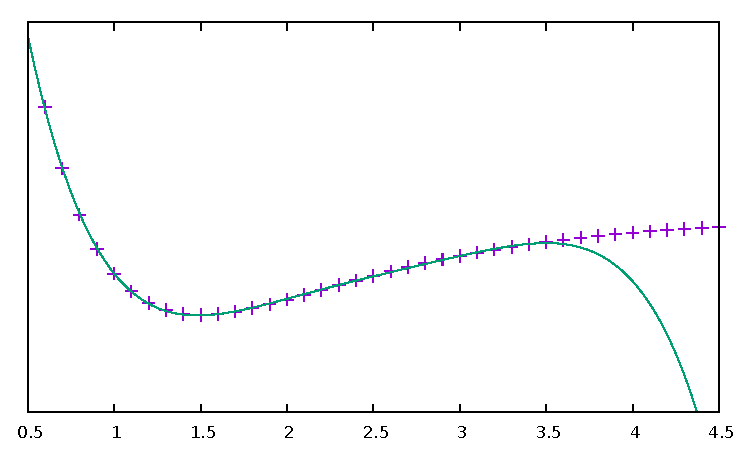
\includegraphics[scale=0.8]{pot_expand} 
	\caption{Illustration of how expansion (line) of actual potential (crosses) can fail.}
	\label{fig:pot_exp}
\end{figure}

\subsection{Number of Atoms and Modes}
The number of atoms and vibrational modes is defined by the keywords
\begin{verbatim}
Natoms n
Nmodes i
\end{verbatim}
where \verb|i| is normally 3\verb|n|$-$6 for non linear molecules and 3\verb|n|$-$5 for linear molecules.

\subsection{Primitive Block}
The polyad number and maximum energy for the primitive basis functions are set in the primitive block:
\begin{verbatim}
PRIMITIVES
Npolyads p
enercut  x
END
\end{verbatim}
As discussed in more detail in later chapters, TROVE uses products of primitive one-dimensional functions as basis functions. 
The polyad number, $P$, is a way to restrict the size of the basis set.\cite{TROVE} 
The sum of the primitive function's vibrational quantum number, $v_i$, is then restricted to be below \verb|n|, that is:
\begin{equation}
\label{eq.polyad}
P = \sum_i a_i v_i \le n.
\end{equation}
where $a_i$ is an integer used to control the basis further.
For fast, test calculations a low value of \verb|n| should be used, for example 4. 
Increasing n gives a larger basis set which will give more accurate results (and extend the energy range) 
at the expense of time and memory.
Note that because of how the polyad number is defined, even increasing \verb|n| by 1 can lead to a much larger basis.

Another way of limiting the size of the primitive basis functions is by energy. 
The \verb|enercut| keyword specifies the maximum energy a primitive basis function can have if it is to be included. 
As discussed below, the basis set is further restricted by energy in the Contraction block and so usually \verb|x|
 is set to a large value. For example 40,000 (in units of wavenumbers, cm$^{-1}$). 

\subsection{Contraction Block}
As will be discussed in later chapters, TROVE builds contracted basis functions from the primitive basis functions. 
In the Contraction block the parameters for making this contraction are chosen. A Contraction block example is 
\begin{verbatim}
CONTRACTION
  Npolyads        n
  enercut         x
  coeff_thresh    1.0d-30
  degeneracy      1d-02
  sample_points   40
  sample_attempts 500
  symm_toler      1.0d-3
END
\end{verbatim}
\verb|Npolyads| is the same as for the Primitive block and defined in equation \ref{eq.polyad} 
and sets the maximum polyad number for the contraction. 
Similar to the primitive block, \verb|enercut| sets the maximum energy a contraction can have. The value of \verb|enercut| chosen depends on the application. 
Because the maximum energy of the contracted basis functions are set, it makes sense to set the value of \verb|enercut| in the Primitive block large.

Also given in the Contraction block are parameters relating to how TROVE works out the symmetry
of contracted basis functions (\verb|coeff_thresh, degeneracy...|). This will be described in later chapters and has been discussed in a recent publication \cite{17YuYaOv.methods}.


\subsection{Symmetry}
The symmetry of the molecule is specified by the \verb|SYMGROUP| keyword. 
The symmetry of a given molecule is set in the .mol file which, as ever, will be discussed in later chapters. 
For PF$_3$ the \verb|SYMGROUP| is set using
\begin{verbatim}
SYMGROUP C3v(M)
\end{verbatim}

\subsection{Diagonalizer Block}
The Diagonalizer block determines the way in which the Hamiltonian matrices are diagonalized. 
The method of carrying out the diagonalization is specified by a keyword related to the LAPACK/BLAS program which are used.
These are standard programs used for carrying out matrix manipulations used in many areas of science, engineering, mathematics,
etc. 
\verb|SYEV| is the default value which computes all eigenvalues and eigenvectors. \verb|SYEVR| allows an uppervalue on the computed eigenvalues to be specified.
There is another keyword, \verb|enermax|, which limits the energies of eigenfunctions which are saved. For example
\begin{verbatim}
DIAGONALIZER
 SYEV
 enermax 16000.0
end
\end{verbatim}
If a pure vibrational calculation (J = 0) is being carried out, 
the energies of excited states are automatically given relative to the zero point energy (ZPE) of the ground vibrational state. 
For J $>$ 0 calculations, the keyword \verb|ZPE| followed by the vibrational zero point energy should be specified 
so that rotational-vibrational energies are also given relative to the ground state.

For large calculations, it is more efficient to diagonalize each symmetry's Hamiltonian matrix separately. The symmetry of 
interest is specified using the keyword \verb|gamma n| where \verb|n|=1,2.. is the symmetry of interest.

\subsection{Print Out Level}

The amount of output printed is specified by the \verb|verbose| keyword. A value of 4 is sufficient for most purposes.
\begin{verbatim}
verbose 4
\end{verbatim}
Increasing this value will produce more output, this is useful for debugging, etc.

\subsection{Specifying the Molecule}
The molecule is defined in TROVE by the following
\begin{verbatim}
dstep            0.01
COORDS           linear
TRANSFORM        r-alpha
MOLTYPE          XY3
MOLECULE         PF3
REFER-CONF       RIGID
\end{verbatim}

\verb|dstep| has to do with how fine a grid TROVE carries out the coordinate transform on.

The \verb|COORDS| keyword specifies the type of internal coordinates. The standard option is \verb|linear| which indicates 
that the kinetic and potential energy should be expanded in linear coordinates \cite{TROVE}. 
Another option is \verb|local| which 
uses curvilinear coordinates \cite{15YaYuxx.method}. Currently curvilinear coordinates are not a part of `standard' TROVE. 

\verb|TRANSFORM| specifies how to transform the coordinates from Z-matrix to the coordinates used in TROVE.
This is specified in the .mol file for the molecule of interest.
For the PF$_3$ example here, the details of the transformation are given in the `r-alpha' subroutine.

As the symmetry transforms only need to specified for each type of molecule of the same symmetry, they can be reused. 
For example PCl$_3$ belongs to the same symmetry
group as PF$_3$. The \verb|MOLTYPE| keyword identifies the `type of molecule' and molecules of the same symmetry can 
then be straightforwardly used. This keyword specifies the subroutine to use to define rotational symmetries, etc.

\verb|MOLECULE| is an optional keyword which specifies the molecule's name.

Whether the molecule is `rigid' or `non-rigid' is specified with the \verb|REFER-CONF| keyword. For non-rigid molecules
a special degree of freedom which is large amplitude (or `floppy') can be specified. Examples include the inversion
motion in ammonia or the torsional motion in ethane. In this case HBJ theory (see Theory chapter) can be used.




\subsection{Z-Matrix Block}
The Z-matrix block specifies the molecule's geometry and masses of atoms. For example for PF$_3$ the Z-matrix is
\begin{verbatim}
ZMAT
    P   0  0  0  0   30.973761998
    F   1  0  0  0   18.998403162
    F   1  2  0  0   18.998403162
    F   1  2  3  0   18.998403162
end
\end{verbatim}
The Z-matrix used by TROVE is very similar to those used by electronic structure programs such as Molpro 
and Gaussian.\cite{06Jensen.book}
The first column is the atom's (element) symbol. The second column is the atom which the atom of that row is connected to. 
The third column is the bond angle between the atom of the row and a specified atom. The fourth column is the dihedral angle 
between the atom of that row and a specified atom. The fifth column has to do with the way a particular molecule type is
set up in TROVE and describes the type of dihedral angle. The sixth column is the atom's mass in atomic mass units. 
Note that isotope masses should be used, not averaged atomic weights. 


\subsection{Basis Block}
The Basis block specifies the type of basis functions used by TROVE and how the kinetic and potential energy is expanded
for each coordinate.
Specifically, the one-dimensional basis functions which will then be used to build up contracted and symmetrized functions. 
An example for PF$_3$ is 
\begin{verbatim}
BASIS
0,'JKtau', Jrot 0
1,'numerov','linear','morse',range 0,7, resc 2.0, points 2000, borders -0.4,2.0
1,'numerov','linear','morse',range 0,7, resc 2.0, points 2000, borders -0.4,2.0
1,'numerov','linear','morse',range 0,7, resc 2.0, points 2000, borders -0.4,2.0
2,'numerov','linear','linear' range 0,14, resc 1.0, points 2000, borders -1.3,1.3
2,'numerov','linear','linear',range 0,14, resc 1.0, points 2000, borders -1.3,1.3
2,'numerov','linear','linear',range 0,14, resc 1.0, points 2000, borders -1.3,1.3
END
\end{verbatim}
The first line in this block, \verb|0,'JKtau', Jrot 0| specifies the rotational functions. 
For $J>0$ calculations the value of \verb|Jrot| is changed to $J$ of interest.
PF$_3$ has $3N - 6 = 3(4) - 6 = 6$ internal degrees of freedom and thus 6 basis functions are required. 
Basis functions are grouped using an integer label.
For this example, '1s' are the P-F stretches and '2s' are the P-F bends. The grouping is used for producing symmetric 
combinations of basis functions and only coordinates symmetrically related should be grouped together. Details of this
procedure are discussed in the Theory chapter and in a recent paper \cite{17YuYaOv.methods}.

For a given basis function row the options are as follows. The first keyword specifies what the one-dimensional basis 
functions are. In this example they are numerically generated using the Numerov-Cooley method. 
Other options are `harmonic' and `morse' where these analytical basis functions shall be used.
The second keyword specifies how the kinetic energy operator is expanded.
The third keyword gives the expansion coordinates for the potential. Here 'Morse coordinates' of the form
 $1 - e^{-\alpha(r-re)}$ are used for the stretching coordinates while `linear' (the angles themselves) 
coordinates are used for the bends.

The numbers after \verb|range| specify the range of vibrational quantum numbers of the one-dimensional functions to be used.
 For the example here, 0-7 is used for stretches and 0-14 for bends.
This is related to the definition of the maximum polyad number used in equation \ref{eq.polyad}. The number after \verb|resc|
gives the waiting of the vibrational quantum number for that coordinate. 
Since the P-F stretches here have a waiting of 2, it only makes sense to generate them from 0-7 if the
polyad number is set to 14.

\verb|points| and \verb|borders| specify the number of points and the starting points for the Numerov-Cooley integration.
Generating these one-dimensional functions is fast and so many points should be taken. 
 The borders should be set far enough into the classically forbidden region of the potential such that 
 the results are not sensitive to slightly larger or lower values. The units for \verb|borders| are the same as those used
that the potential was expanded in (Morse for stretches and angles in radians for bends in this example).

The details of the primitive basis sets are given in the TROVE output file and will be discussed in 
Chapter \ref{chap:outputs}.

\subsection{Checkpoint Block}
The Checkpoint block determines which checkpoint files are saved by TROVE. 
This is an important aspect of TROVE as usually calculations are built up sequentially. 
The checkpoint files allow a calculation to be restarted with the results of previous calculations read in by TROVE. 
For each keyword in the Checkpoint block the options are `read' or `save'. 
If `read' is specified then the checkpoint file (.chk) associated with that keyword must be present in the directory 
where the calculation is run. 
In this case that file will be read in for TROVE to use. If `save' is specified then the checkpoint file associated with 
that keyword will be saved.

The hamiltonian.chk file contains details of the kinetic and potential energy expansion, controlled by the \verb|Kinorder| and 
\verb|Potorder| keywords discussed above. The associated keyword is \verb|hamiltonian|. 
Alternatively the keywords \verb|kinetic| and \verb|potential| can be specified 
but if set to save, still generate hamiltonian.chk. 
This is usually the first part of a TROVE calculation. Once the hamiltonian.chk file is generated to a sufficient order 
(for example 6/8 for kin/pot order) it can be reused while different basis sets, polyads, etc are compared. 

If transition moments or intensity calculations are being carried out then the keyword \verb|external| should be included 
and set to save. This generates an expansion of the dipole moment surface (DMS) and requires a DMS to be provided. 

The primitive basis set can be saved/read with the \verb|basis_set| keyword. This will generate .chk files with the
one dimensional numerov and contracted primitive basis functions. This is also included if the `hamiltonian' keyword is used. 
The contracted basis is saved/read with the \verb|contract| keyword and generates a \verb|contr_vectors.chk| 
checkpoint file and human readable file \verb|contr_descr.chk|.

The matrix elements of the Hamiltonian between contracted functions can be saved using the \verb|matelem| keyword. The file 
\verb|contr_matelem.chk| is generated. This can be very large depending on the basis set.
Similarly, vibrational elements of the DMS can be saved using the keyword \verb|extmatelem| 
which generates the \verb|contr_extfield.chk| file. 

If the eigenfunction of the calculation are required (for example for transition moment calculations) 
then the \verb|EIGENFUNC| keyword should be set to save. 
This generates \verb|eigen_vectors[J].chk| files and human readable \verb|eigen_descr[J].chk| files, where J is the rotational
quantum number. The eigenfunctions are used to for generating basis functions for J$>$0 calculations as discussed below. 

A description of how these files are used for J$>$0 calculations is given below.


\subsection{Equilibrium Block}
The Equilibrium block specifies the equilibrium bond lengths (in Angstrom) and bond angles of the molecule. 
TROVE uses these values
to calculate Cartesian coordinates and transform between coordinate systems. For PF$_3$ this is
\begin{verbatim}
EQUILIBRIUM
Re          0       1.56
Re          0       1.56
Re          0       1.56
alphae      0     98.000 deg
alphae      0     98.000 deg
alphae      0     98.000 deg
end
\end{verbatim}



\subsection{Specparam Block}
The Specparam block is used to define special parameters. For example, the value of $\alpha$ in the Morse potential 
function.


\subsection{Poten Block}
The Poten block is used to specify the PES. For PF$_3$ the first few lines are 
\begin{verbatim}
POTEN
NPARAM   304
POT_TYPE  poten_xy3_morbid_10
COEFF  list  (powers or list)
VE                      0                   0.000000000000
FA1                     1               -5730.010012350451
FA2                     1             1091683.728331340943
FA3                     1            -1947258.254744407022
.
.
.
\end{verbatim}
\verb|NPARAM| is used to specify the number of parameters used to define the PES. 
\verb|POT_TYPE| is the name of the potential energy surface being used which is defined in
the .mol file. The \verb|COEFF| keyword specifies whether the potential is given as a simple list or if the powers or the 
expansion are given. This depends on how the potential has been set up. The list of PES parameters is then given. 

\subsection{External Block}
The External block is similar to the Potential block but defines other functions to be included in the calculations. Most 
commonly this will be the dipole moment surface (DMS). For example for 
PF$_3$ the first few lines are 
\begin{verbatim}
DIPOLE
rank 3
NPARAM  127 0 0
DMS_TYPE  XY3_MB
COEFF   list
dstep   0.005
COORDS  linear
Order   6
parameters
 charge                  0                  0.0
 order                   0                  4.0
 alphae                  0                  98.000000000000
 re14                    0                   1.560000000000
 beta                    0                   1.000000000000
 gamma                   0                   0.000000000000
 delta                   0                   0.000000000000
 mu0                     1                  -0.177517341983
 F1                      1                  -2.287669265640
.
\end{verbatim}
As the DMS is a vector function (it has values for the x, y and z directions) the three numbers of parameters 
for each is specified in \verb|nparam|. For PF$_3$ only one direction is needed however due to the way the DMS is specified.
The name of the DMS is specifed by \verb|DMS_TYPE| which corresponds to the name in the .mol file.
\verb|COEFF| specifies how the parameters are given (a list in this case) 
and \verb|COORDS| is used to describe which coordinates are used to expand the dipole in TROVE. \verb|Order| specifies
the order to expand the dipole to, similar to the keywords for the kinetic and potential energy.
The list of parameters is then given in a similar way to the Poten block. 

The external block is also used to refine potential energy surfaces as discussed in the Refinement chapter. It can 
even be used for more exotic applications such as introducing quadrupole potentials, etc but this will not be 
covered here.


\subsection{Intensity Block}
As described below, once eigenfunction for the vibrational and rotational states are calculated, 
they can be used to calculate the intensity of transitions.
Options for controlling this in TROVE are specified in the Intensity block. 

Transition moments (TMs) can be calculated once vibrational ($J=0$) eigenfunctions are available (see below). 
In this case the Intensity block is given, for example
\begin{verbatim}
 INTENSITY
  tm
  THRESH_TM  1e-12
  ZPE          11014.221565
  selection (rules) 1 1 1 1 1 1 1 1  (N of irreps)
  J,  0,0
  freq-window  -0.0001,   5000.0
  energy low   -0.0001,  2000.0, upper   -0.00, 7000.0
  END
\end{verbatim}
\verb|tm| tells TROVE to calculate transition moments only. \verb|THRESH_TM| sets the threshold for the smallest
TMs to be calculated.
\verb|ZPE| is the value of the molecule's zero-point energy. 


For calculating absorption intensities the Intensity block takes the following form
\begin{verbatim}
 INTENSITY
  absorption
  THRESH_INTES  1e-20
  THRESH_LINE   1e-20
  THRESH_COEFF  1e-18
  TEMPERATURE   300.0
  Partition     1000.0
  GNS          8.0 8.0 8.0
  ZPE          11014.221565
  selection (rules) 1 1 2  (N of irreps)
  J,  0,10
  freq-window  -0.1,   4000.0
  energy low   -0.1,  2000.0, upper   -0.1, 6000.0
END
\end{verbatim}
\verb|absorption| specifies that absorption intensities between states are to be calculated.


\verb|THRESH_INTES/LINE/COEFF| are used to control the level of print out for intensities. Very large outputs
can be produced if these are set very low (as needed for `production' quality line lists) but for 
quicker checks higher values should be used.


\verb|TEMPERATURE| is used to specify the temperature of interest. This will affect the population of states 
(Boltzmann population).


\verb|Partition| is the value of the partition function. 
This can be calculated from all of the ro-vibrational energy levels used. 
Note that at high temperatures enough energy levels must be included for accurate results. 
If this is not the case (for example, for a test calculation) then a literature value could be used.


\verb|GNS| is the spin statistical weights for each symmetry. 
These can be looked up for many molecules or worked out from the procedure in Bunker and Jensen, chapter 8 \cite{98BuJexx}.
\verb|selection| is used to specify which symmetries can make up the initial and final states of a transition.
The product of the upper and lower eigenfunctions must contain a component of the dipole itself \cite{98BuJexx}. Thus for the PF$_3$
example, A$_1$ and A$_2$ are grouped together while E can only go to E. Integers are used to form groups, in this case
1 1 are for A$_1$ and A$_2$ and 2 is for E.


\verb|J,  i,j| specifies the rotational states to be included. In the example above 0 to 10 were used. It is often 
better to split a calculation into 0,1-1,2-2,3, etc to fit into time allocations on computers.
The vibrational states to be included can also be specified by the \verb|v i, lower x, y, upper x', y'| 
where i is the number of a vibrational mode and x, x' and y, y' give the 
limits for the lower and upper states included. If this is not included then all vibrational states are considered. 


\verb|freq-window| This specifies the frequency window (in wavenumbers) in the spectra to be used. 
In the example here -0.1 is used as the minimum to guarantee values from 0 are used while 4000 is the maximum considered. 
\verb|energy low| specifies the energies of the lower and upper states to be included. In the example the highest energy lower state to include it 2000 so since the maximum frequency of light considered is 4000, the upper state needs a maximum of 6000 (energy proportional to frequency, $E = h \nu$).

To calculate absorption intensities the eigenfunctions and eigenvalue files of the states to be included must be included 
in the directory where TROVE is run. More on this will be described below. 

The working equations for intensity calculations are discussed in the Theory chapter.




\section{Practical Guide to Running TROVE}
In this section the recommended steps for using TROVE are described, 
from calculating vibrational energies up to rotational-vibrational absorption intensities. 
It will be assumed that the PES and DMS are available and that the symmetry group, Z-matrix, 
primitive basis set, etc have been set up. These inputs are generally fixed
once they have been decided on and typically the user does not need to modify them.

This section can be followed most easily in conjunction with the TROVE training directory which should come
with this manual. This contains a TROVE executable file and inputs, outputs and checkpoints for a model
PF$_3$ calculation as well as a README file. It may be necessary to compile a version of TROVE on the local 
computer to get working executable. 

The first step in any TROVE calculation is the production of the hamiltonian.chk checkpoint file. 
As discussed above, this contains the details of the kinetic and PES expansion 
and if required, the DMS expansion, which are used in later parts of TROVE. 
In the Checkpoint block the following should be set to save
\begin{verbatim}
kinetic     save
potential   save
(external   save)
\end{verbatim}
This will generate the hamiltonian.chk file which will be read in subsequent calculations. 
The time taken and memory usage of this step can vary
depending on the expansion orders of the kinetic energy, PES and DMS. 
As mentioned above, low expansion orders (for example 2 and 4 for kinetic and potential respectively) 
are useful for test calculations but are not very accurate but larger expansions (e.g 6 and 8) 
take a longer time to compute and use. 

The basis set checkpoint files are usually generated next. In the Checkpoint block this is specified by
\begin{verbatim}
basis_set   save
CONTRACT    save
\end{verbatim}
The \verb|basis_set| keyword generates the file \verb|prim_bset.chk| and, if a Numerov basis is selected,
 \verb|numerov_bset.chk|. 
\verb|CONTRACT| generates the file \verb|contr_vectors.chk| which contains the contracted basis functions. 
This also generates the file \verb|contr_matelem.chk| which contains 
vibrational matrix elements of the Hamiltonian in the contracted basis representation.
 Depending on the size of the basis set, this file can be very large.
The human readable files \verb|contr_descr.chk| and \verb|contr_quanta.chk| are also generated which contain descriptions of
the contracted basis functions and of the energies corresponding to the contracted basis functions.

It is also possible instead to use the \verb|Hamiltonian| keyword. If this is set to save then the kinetic and potential expansion and primitive basis set will be generated.

At this stage, TROVE will calculate and output the vibrational energies. The eigenfunctions for each vibrational state are saved using
\begin{verbatim}
EIGENFUNC   save
\end{verbatim}
These are used in subsequent transition moment and absorption intensity calculations.
 A series of files, \verb|eigen_vectors0_n.chk| are generated where n ranges from 1 to however
many symmetry classes there are for the molecule of interest.
 Similar to the contracted basis, \verb|eigen_desc0_n.chk| human readable files for each symmetry class of 
eigenvectors are also generated along with \verb|eigen_quanta0.chk| which contains a description of eigenvectors and eigenvalues.

The steps described above can all be carried out with a single run of TROVE, setting all of the keywords to save. 
For large calculations however, it is usually best to build up the checkpoint files, checking each step is successful. 
To follow the steps outlined above, the keywords should be set to read for .chk files which have already 
been generated. For example, once the \verb|hamiltonian.chk| file is generated, \verb|kinetic| and \verb|potential| 
can be set to read.

Once the \verb|contr_matelem.chk| file has been created along with vibrational eigenfunctions, 
it is in principle possible to calculate J$>0$ energies. 
A faster and more efficient way to do this however is to make
use of the `J=0 representation'. This is where the vibrational eigenfunctions for J=0 calculation 
are used as a basis set for J$>0$ calculations.\cite{jt466} This usually leads to much faster
calculations of excited rotational states. 
To use this method put \verb|model j=0| anywhere in the Contraction block and in the Checkpoint block put
\begin{verbatim}
CONTRACT    save
matelem     convert
(extmatelem  convert)
\end{verbatim}
This will produce a new file, \verb|j0_matelem.chk| and, if extmatelem specified, \verb|j0_extfield.chk|. 
\verb|j0contr_descr.chk|, \verb|j0contr_quanta.chk| and
\verb|j0contr_vectors.chk| files are also generated, equivalent to those described above. A $J=0$ calculation should then 
be run setting \verb|CONTRACT| and \verb|matelem| to read and \verb|EIGENFUNC| save. This will produce a desc and checkpoint
files for the $J=0$ eigenfunctions but saved in the J=0 representation. 

Once these files have been generated it is then straightforward to carry out calculations for $J>0$. In the Basis block change
\begin{verbatim}
0,'JKtau', Jrot 0 
\end{verbatim}
to 
\begin{verbatim}
0,'JKtau', Jrot 1
\end{verbatim}
(or whatever J of interest). 
The \verb|model j=0| keyword should be left in the Contraction block. In the Diagonalizer block the keyword ZPE should 
be added to set the vibrational zero point energy. 
The ro-vibrational energy levels will then be given with respect to this. 
In the Checkpoint block everything should be set to read apart from \verb|EIGENFUNC| if the rotational 
eigenfunctions are required. 


Transition moments can be calculated by inserting the Intensity block into the input file as described above. 
The directory in which TROVE is run should contain the vibrational
eigenfunctions stored either in the standard contracted form 
(\verb|eigen_vectors0.chk,|) or the J=0 form (\verb|J0eigen_vectors0.chk|). 

Absorption intensities (line lists) can be calculated once the rotational-vibrational 
eigenfunctions of interest have been calculated, usually using the J=0 method. 
The relevant .chk files describing the eigenfunctions should all be present in the directory where TROVE is run. 
The Intensity block should be included in the input block with the \verb|absorption| keyword as described above.

For both transition moment and absorption intensity calculations everything should be set to read in the Checkpoint block 
(with the relevant checkpoint files included in the directory). 

Although TROVE can calculate intensities, the GPU program GAIN can do this far faster.\cite{jt653} 
The use of the program will be described in Chapter \ref{chap:linelists} but the input is the same as described above. 


\section{Sample TROVE Input File}

Below is a sample TROVE input file for the molecule PF$_3$. Using this file (and adding in Intensity blocks when needed)
a full line list for this molecule could be produced. To save space the PES and DMS parameters have not been included
in full. The actual text file should be kept in the same directory as this manual.

\begin{verbatim}

mem 20 gb


KinOrder  6 (Max order in the kinetic energy expansion)
PotOrder  8 (Max order in the potential energy expansion)


Natoms 4    (Number of atoms)
Nmodes 6    (Number of modes = 3*Natoms-6)


(ACTIVE SPACE CUTOFFS:)

PRIMITIVES
  Npolyads         14   (how many polyads we calculate)
  enercut        100000.(energy cut in the primitive matrix for the diagonalization)
END

CONTRACTION
  Npolyads         14    (how many polyads in the contracted represent.)
  enercut       100000.  (energy cut in the primitive matrix for the diagonalization)
  degeneracy    1e-3     (threshold to define degeneracy)
  sample_points  40
  sample_attempts 500
  symm_toler      1e-3
  coeff_thresh    1e-16
  fast_ci
  exp_coeff_thresh   1.0d-8
END


verbose 3


DIAGONALIZER
 SYEV
end


dstep 0.01    (finite difference element for each mode )
TRANSFORM  r-alpha
MOLTYPE    XY3
MOLECULE   PF3
COORDS     linear
REFER-CONF RIGID  (Reference configuarion: RIGID or NON-RIGID)


SYMGROUP C3v(M)


ZMAT
    P   0  0  0  0   30.973761998
    F   1  0  0  0   18.998403162
    F   1  2  0  0   18.998403162
    F   1  2  3  0   18.998403162
end

CHECK_POINT
HAMILTONIAN none
kinetic     save
potential   save
external    none
basis_set   save
CONTRACT    save
contr-ci    save
EIGENFUNC   none
matelem     save 
extmatelem  none
END




BASIS
  0,'JKtau', Jrot 0
  1,'numerov','linear','morse',range 0,7,resc 2.0,points 2000, borders -0.4,2.0
  1,'numerov','linear','morse',range 0,7,resc 2.0, points 2000, borders -0.4,2.0
  1,'numerov','linear','morse',range 0,7, resc 2.0, points 2000, borders -0.4,2.0
  2,'numerov','linear','linear',range 0,14,resc 1.0, points 2000, borders -1.3,1.3
  2,'numerov','linear','linear',range 0,14,resc 1.0, points 2000, borders -1.3,1.3
  2,'numerov','linear','linear',range 0,14,resc 1.0, points 2000, borders -1.3,1.3
END

EQUILIBRIUM
Re          0       1.56
Re          0       1.56
Re          0       1.56
alphae      0     98.000 deg
alphae      0     98.000 deg
alphae      0     98.000 deg
end



SPECPARAM
beta        0        1.00000
beta        0        1.00000
beta        0        1.00000
END

POTEN
NPARAM   304
POT_TYPE  poten_xy3_morbid_10
COEFF  list  (powers or list)
VE                      0                   0.000000000000
FA1                     1               -5730.010012350451
FA2                     1             1091683.728331340943
FA3                     1            -1947258.254744407022
FA4                     1            18286059.212070591748
FA5                     1          -105327110.803434416652
.
.
.
.
end
        

DIPOLE
rank 3
NPARAM  127 0 0
DMS_TYPE  XY3_MB
COEFF   list
dstep   0.005
COORDS  linear
Order   6
parameters
 charge                  0                  0.0
 order                   0                  4.0
 alphae                  0                  98.000000000000
 re14                    0                   1.560000000000
 beta                    0                   1.000000000000
 gamma                   0                   0.000000000000
 delta                   0                   0.000000000000
 mu0                     1                  -0.177517341983
 F1                      1                  -2.287669265640
 F3                      1                   0.432166856494
 F4                      1                  -0.037093470208
 F5                      1                  -0.761988732763
 .
 .
 .
 .


\end{verbatim}












